\hypertarget{ch2}{%
\chapter{Physiographic controls and sensitivities of midwinter snowpack in Sierra Nevada, CA}\label{ch2}}

\hypertarget{ch2-abstract}{\section{Abstract}\label{ch2-abstract}}

%==============================================================================
%==============================================================================
%==============================================================================
\hypertarget{ch2-intro}{\section{Introduction}\label{ch2-intro}}
\subsection{Significance and Motivation}
Seasonal snowmelt from midlatitude mountain environments is the main source of water for nearly a billion people across the globe \citep{sturmWaterLifeSnow2017}.
Climate warming is affecting the stationarity of various hydroclimatic processes \citep{millyStationarityDeadWhither2008}. In the Western US (WUS), this means warmer winter temperatures \cite{gergelEffectsClimateChange2017}, more cold season precipitation falling as rain \citep{knowlesTrendsSnowfallRainfall2006}, which in turn impact snow accumulation and ablation processes \citep{kapnickCausesRecentChanges2012}. These snowpack variations influence streamflow timing \citep{stewartChangesSnowmeltRunoff2004} and affect the magnitude of streamflow overall \citep{barnhartSnowmeltRateDictates2016}. (***rework). Hydroclimatic changes pose significant implications for water resources management in an uncertain future \citep{livnehDroughtLessPredictable2020}.

Common snow metrics like April 1st snow water equivalent (SWE) and maximum SWE (MSWE) are used to estimate spring flows (**cite). With recent climate change, midwinter melt events caused by snow droughts \citep{harpoldDefiningSnowDrought2017} and dry spells \citep{hatchettMidwinterDrySpells2023} are becoming more common. This melt impacts MSWE, ablation season processes, and streamflow generation. Both \cite{harpoldHumidityDeterminesSnowpack2018} and \cite{musselmanWinterMeltTrends2021} showed the importance of midwinter melt, but their studies relied on station data. Specifically, \cite{musselmanWinterMeltTrends2021} states that to better understand the impact of anthropogenic warming on snow, it is important to continue investigating the relationship between climatology, physiography, and snowpack. This allows for more insight into how snowpack will react to warming temperatures across spatial scales, as this still remain unclear \citep{molotchEstimatingDistributionSnow2008}. Therefore, we must quantify the physiographic controls and climatological sensitivities of hydrologically important snowpack metrics.

% 
\subsection{Background}
\subsubsection{Key physiographic parameters}
Physiographic parameters (i.e., elevation, aspect, slope) are first order controls of fluxes of water, energy, and nutrients through the environment \citep{pelletierWhichWayYou2018a}. Aspect, or slope orientation, serves as a primary control on hydrologic, ecologic, and geomporphic processes, as it moderates the intensity of incoming solar radiation (herein insolation) \citep{broxtonRoleAspectQuantify2009}. Net shortwave radiation is the primary driver of snowmelt in the ablation season \citep{marksClimateEnergyExchange1992a}. This process is magnified in midlatitude mountain environments, where the lower sun angles create a greater difference between north and south-facing slopes. 

\subsubsection{Limitations of previous work}
Spatial and temporal scales of observations need to be relevant to the physical process of interest. For instance, \cite{bloschlScalingIssuesSnow1999} showed that the relevant spatial scale for snow hydrology in mountain regions $\sim$100~m, with this resolution showing the ability to resolve critical spatial characteristics. **Need the right scales for both measurements and models.  AND, we need to consider the spatial and temporal scales for understanding processes.** Past studies have leveraged long-term point-based in situ data \citep{clowChangesTimingSnowmelt2010,harpoldChangesSnowpackAccumulation2012a,kapnickCausesRecentChanges2012,musselmanWinterMeltTrends2021} and kilometer-scale models to evaluate various climatic-scale monotonic snowpack metric trends 
\citep{moteDECLININGMOUNTAINSNOWPACK2005, moteDramaticDeclinesSnowpack2018, zengSnowpackChange19822018, haleDriversSpatiotemporalPatterns2023}. However, snow pillows cover less than 1~\% of the land area and are limited to mainly mid-elevation flat forest cuts \citep{guan20102011Snow2013}. Macroscale hydrologic models (e.g., Variable Infiltration Capacity (VIC) \citep{liangSimpleHydrologicallyBased1994}) or snow reanalyses (e.g. UA daily 4~km SWE product \citep{broxtonLinkingSnowfallSnow2016}, SNOw Data Assimilation System (SNODAS) \citep{barrettNationalOperationalHydrologic2003}) have resolutions on the scale of kilometers. This makes neither of these data well-suited for understanding snowpack patterns in complex topography. \cite{trujilloSnowpackRegimesWestern2014} used SNOTEL data from the WUS to characterize distinct geographic snowpack regimes, yet physiographic variables were not considered due to data limitations.

%%% studies that do use aspect! (elder???)
Past studies have considered physiography in their characterization of mountain snowpack. \cite{pomeroyVariationSurfaceEnergetics2003} used in situ meteorologic instrumentation setup slope normal instead of the traditional gravimetric orientation and found marked differences in insolation and ablation rates on south and north-facing slopes. Lidar data has been employed to investigate snow depth variation with respect to various landscape characteristics \citep{kirchnerLiDARMeasurementSeasonal2014, tennantRegionalSensitivitiesSeasonal2017}. Various snow modeling studies have considered physiographic effects on snowpack accumulation and ablation \citep{broxtonForestCoverTopography2020,mazzottiCanopyStructureTopography2023, lopez-morenoEffectSlopeAspect2014}. However, all the studies referenced are limited by either their small spatial scale or short temporal scale.

\subsection{Study Overview}
Here, we use the Sierra Nevada Snow Reanalysis (SNSR), a 90~m spatiotemporally continuous SWE data set from 1985--2016 (32 years), for a comparison of how snowpack metrics change with physiography, specifically aspect and elevation. This novel dataset addresses two of the main deficiencies outlined above: it is high-resolution (90~m) spatially distributed data that spans a 32-year study period. 

We analyze four snowpack metrics: MSWE, day of MSWE (DOM), fraction of snow ablation before 1 April (FM) \citep{musselmanWinterMeltTrends2021}, and amount of midwinter snow ablation (MWA) \citep{harpoldHumidityDeterminesSnowpack2018}. Our study aims to answer the following research questions:

\begin{enumerate}
    \item How does midwinter ablation vary across a watershed with respect to physiography?

    \item Does midwinter ablation explain the differences in MSWE across the landscape?
    
    \item What are the physical mechanisms driving this variation in midwinter ablation?
\end{enumerate}



%=========================================================================
%=========================================================================
%=========================================================================
\hypertarget{ch2-sa}{\section{Methods}\label{ch2-sa}}

--descrition of overall approach
--this is an semi-empirical study using gridded SWE and climate data based on in situ obersations, which are interporlated across space.***

\hypertarget{ch2-sa}{\subsection{Study Area}\label{ch2-sa}}

% We selected three watersheds to analyze: the Yuba, Upper San Joaquin (USJ), and the Kern. These basins were selected as they span a range of latitudes, forest cover, and elevation. The basins were segmented into five elevation zones (EZs): EZ1 (1500--1900~m), EZ2 (1900--2300~m), EZ3 (2300--2700~m), EZ4 (2700--3100~m), and EZ5(3100--4361~m). EZ1--4 are split into even 400-m segments, while EZ5 extends from 3100~m to the maximum elevation (4361~m). EZ5 was chosen to be larger to simplify our results, as we found that areas above 3100~m exhibited similar snow metric characteristics. 

% The basins were then segmented into north-facing (315--45$^{\circ}$) and south-facing (135--215$^{\circ}$) aspects, with a least a slope of >~4$^{\circ}$ needed to be considered in our analysis. By setting this slope threshold, we ensure that only complex mountain terrain, and flatter areas. The north south 

%%% add in table
- basin total area, elevation range, cc \%, percent area north-facing and south-facing, percent area "seasonal snow" as we define

%f1
\begin{figure*}[t]
\centering
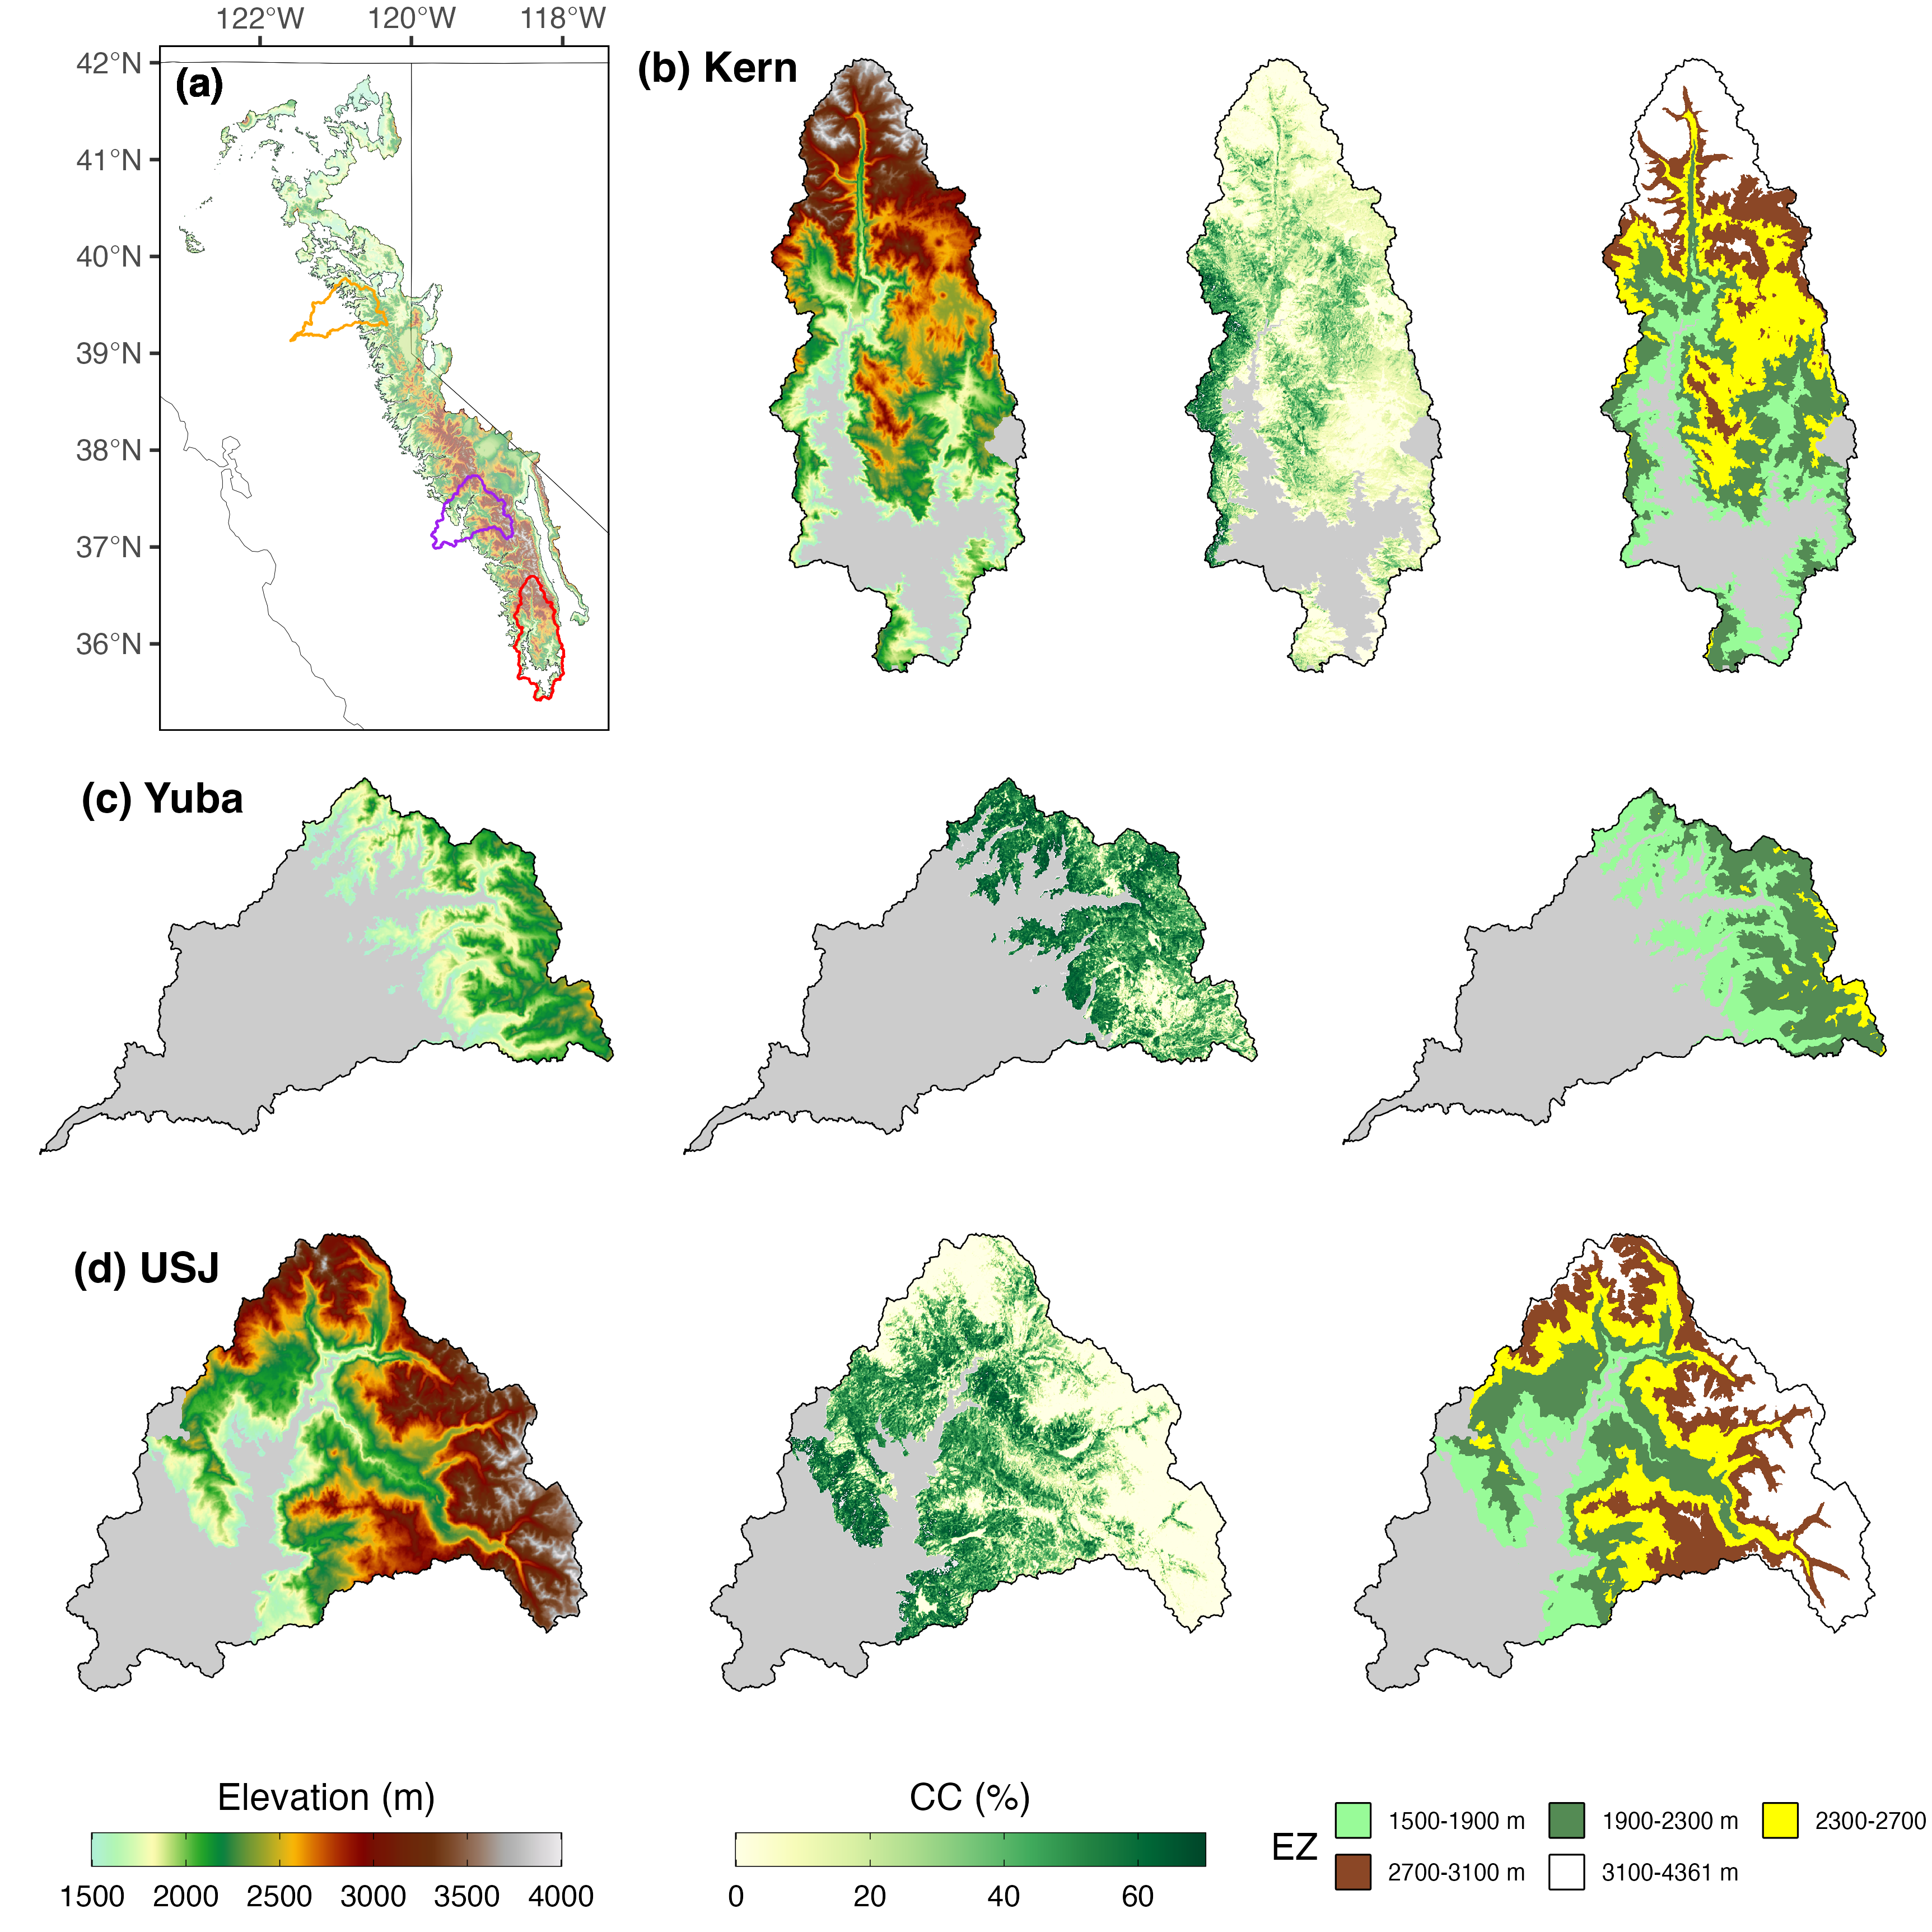
\includegraphics[width=14cm]{figures/ch2_figs/kuy_study_area_v2.png}
\caption{\textbf{(a)} The full extent of the SNSR study domain with Yuba (orange), USJ (purple), and Kern (red) basins shown. From left to right for the \textbf{(b)}~Kern, \textbf{(c)}~Yuba, \textbf{(d)}~USJ: elevation, canopy cover (\%), and elevation zones (EZs).}
\label{kuy_study_area}
\end{figure*}
%==============================================================================
\hypertarget{ch2-sa-1}{\subsubsection{Yuba}\label{ch2-sa-1}}

-info veg, reference table i need to make, the main channels, water managments

%==============================================================================
\hypertarget{ch2-sa-2}{\subsubsection{USJ}\label{ch2-sa-2}}


%==============================================================================
\hypertarget{ch2-sa-3}{\subsubsection{Kern}\label{ch2-sa-3}}


%==============================================================================
%==============================================================================
%==============================================================================
\hypertarget{ch2-do-1}{\subsection{Data Overview}\label{ch2-do-1}}

In this section, we describe the gridded snow reanalysis, meteorologic data, and in situ snow data used in this study.

%==============================================================================
\hypertarget{ch2-do-2}{\subsubsection{SNSR}\label{ch2-do-2}}


The SNSR \citep{margulisLandsatEraSierraNevada2016} is a 90~m gridded daily SWE product for California Sierra Nevada from water year (WY) 1985--2016. These data were created using a Bayesian particle batch smoother data assimilation (DA) technique to retroactively assimilate Landsat fractional snow-covered area (fSCA) with downscaled National Land Data Assimilation System (NLDAS) meteorologic forcing. The MSWE estimates were validated with over 9000 years of snow pillow and snow course data. Detailed information on the development and implementation of this methodology can be found in a series of past publications: \cite{durandBayesianApproachSnow2008, girottoExaminingSpatialTemporal2014, girottoProbabilisticSWEReanalysis2014, margulisParticleBatchSmoother2015}. A recent analysis from \citep{yangIntercomparisonSnowWater2023} evaluated the uncertainty of various SWE products using ASO lidar data. They found that the SNSR performed the best according to various error metrics, making it a well-suited dataset for our analysis.

\hypertarget{ch2-do-2}{\subsubsection{SNOTEL data}\label{ch2-do-2}}


SWE data from 29 SNOTEL sites totaling $\sim$840 station years (Fig. \ref{kuy_study_area}(**UPDATE map with SNOTEL LOCATIONS AND ASPECTS) was used for model validaiton. Operated by the United States Department of Agriculture's Natural Resources Conservation Service (NRCS), it is a comprehensive network of remote, long-term, automated sites spread across the western United States and Alaska. These data are quality controlled by the NRCS.

\hypertarget{ch2-do-2}{\subsubsection{gridMET Data}\label{ch2-do-2}}

We used 4~km meteorological data from gridMET \citep{abatzoglouDevelopmentGriddedSurface2013} to calculate annual (1985--2016) cold season values from October 1 to March 31 (ONDJFM) for three meteorologic variables: mean temperature (T\textsubscript{mean}), relative humidity (RH\textsubscript{mean}), and incoming solar radiation (insolation). Daily ONDJFM where averaged to create the annual metrics. These data were bilinearly downscaled to the 90~m SNSR resolution. Since gridMET does not include a T\textsubscript{mean} or RH\textsubscript{mean} value---only the daily maximum and minimum---these values were averaged to create the two mean variables. Insolation from gridMET is estimated with respect to a planar surface and not topographically corrected. 

%===========================================================================
\hypertarget{ch2-do-2}{\subsubsection{Clear sky insolation}\label{ch2-do-2}}


We estimated 90~m spatially distributed mean ONDJFM clear sky incoming solar radiation (CS insolation) using the R package “insol”, which is based on the Bird model \citep{birdReviewEvaluationImprovement1981}. The model uses the SNSR 90 m DEM as input and accounts for slope, aspect, differential shading, day of year, solar zenith angle, air temperature, elevation, and relative humidity. To calculate CS insolation, the daily values were averaged in the same fashion as the gridMET data. This produced a single estimate, not a time series like gridMET data. CS insolation does not account for cloud cover or variations in latitude in the dataset.


%==============================================================================
%==============================================================================
%==============================================================================

\hypertarget{ch2-methods-1}{\subsection{Snow metric creation and validation}\label{ch2-methods-1}}

\begin{figure*}[t]
\centering
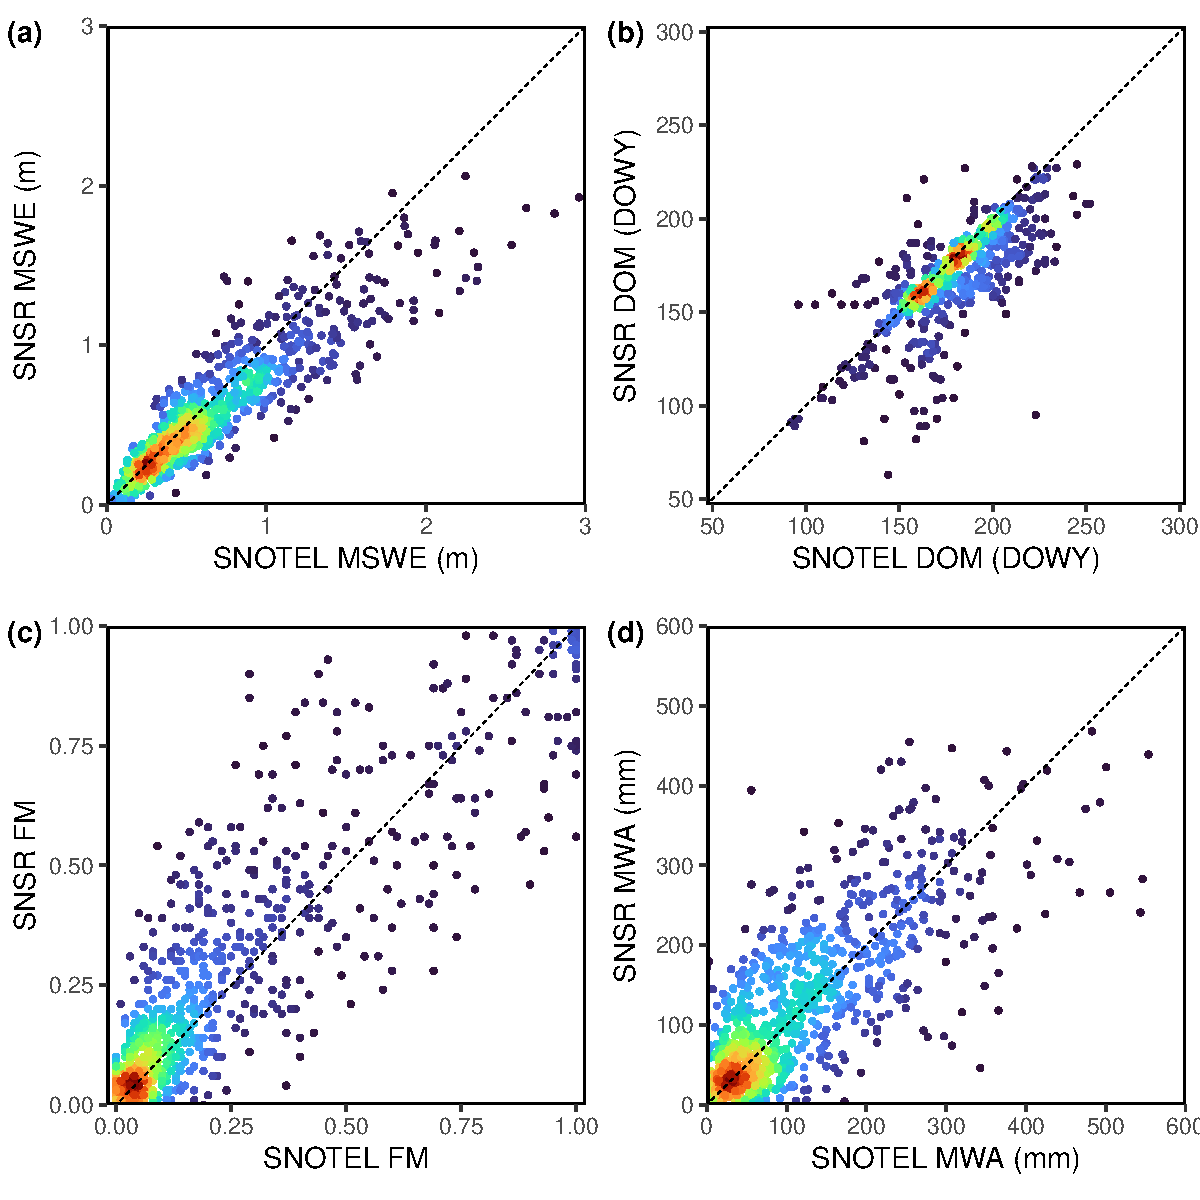
\includegraphics[width=10cm]{figures/ch2_figs/snsr_snotel_metric_compare_new_v1.pdf}
\caption{Density plots comparing SNSR and SNOTEL \textbf{(a)} MSWE, \textbf{(b)} DOM, \textbf{(c)} FM days, \textbf{(d)} MWA for 29 SNOTEL stations from WY 1985--2016 (n $\approx$ 840).}
\label{kuy_study_area}
\end{figure*}

Using the SNSR, we generated four pixel-wise snowpack metrics: MSWE, DOM, FM, and MWA. MSWE is defined as the maximum amount (mm) of SWE in a given pixel for WY, while DOM is the last day of the water year in which the pixel has that amount. As defined \cite{musselmanWinterMeltTrends2021}, FM is the fraction of ablation (e.g., melt, wind transport, sublimation, evaporation) that occurs before April 1st. MWA is the amount of SWE lost in (mm) during the same time period. Reporting both FM and MWA allows for a more complete understanding of midwinter ablation dynamics, as they provide both a fraction and a magnitude.

We focused our analysis on the seasonal snow zone, which is loosely defined as areas that receive snow for the majority of years. To do this, an annual accumulation threshold of 26~mm ($\sim$1~in) of SWE was set for a given pixel to be included. Then, within the 32-year time series, a pixel must meet this condition for at least 27 of the 32 years. *** figure here***?

These metrics were then validated against 29 SNOTEL stations totaling $\sim$840 station years (Figure \ref{kuy_study_area}). SNSR values were selected by the specific pixel in which the SNOTEL station fell. Two correlation coefficients (R and R$^{2}$), root-mean-square error (RMSE), mean absolute error (MAE), mean error (ME), and percent bias (PB) are in Table \ref{tab:snow_metrics_val_table}.

\begin{table}[htbp]
  \centering
  \caption{Error statistics (RMSE, MAE, ME, and PB) and correlation coefficients for (R and R$^{2}$) for the MSWE, DOM, and FM compared to 29 SNOTEL stations from WY 1985–-2016 (n $\approx$ 840). The in situ data are compared against the single SNSR pixel in which the station falls within.}
  \label{tab:snow_metrics_val_table}
  \begin{tabular}{lllllll}
    \toprule
    Snow Metric & R & R$^{2}$ & RMSE & MAE & ME & PB (\%) \\
    \midrule
    Max SWE (m) & 0.9 & 0.81 & 0.22 & 0.15 & $-$0.08 & $-$11.6 \\
    Max SWE (DOWY) & 0.75 & 0.56 & 18.95 & 11.59 & $-$8.05 & $-$4.5 \\
    FM & 0.88 & 0.77 & 0.14 & 0.09 & 0.03 & 12.5 \\
    MWA (mm) & 0.75 & 0.56 & 71.78 & 52.44 & 9.06 & 7.4 \\
    \bottomrule
  \end{tabular}
\end{table}

\hypertarget{ch2-methods-2}{\subsection{Physiographic disaggregation}\label{ch2-methods-2}}

We disaggregated the basins by their physiographic characteristics (elevation, slope, and aspect) in order to understand the relationship between these physical attributes, snow metrics, and climate. This segmenting also controls for precipitation inputs, where we assume that snowfall amounts are relatively constant throughout the EZs. The basins were segmented into five elevation zones (EZs): EZ1 (1500--1900~m), EZ2 (1900--2300~m), EZ3 (2300--2700~m), EZ4 (2700--3100~m), and EZ5 (3100--4361~m). EZ1--4 are split into even 400-m segments, while EZ5 extends from 3100~m to the maximum elevation (4361~m). EZ5 was chosen to be larger to simplify our results, as we found that areas above 3100~m exhibited similar snow metric characteristics. 

The basins were then segmented in north-facing (315--45$^{\circ}$) and south-facing (135--215$^{\circ}$) aspects, with a least a slope of > 4$^{\circ}$ needed to be considered in our analysis. By setting this slope threshold, we focus our analysis on only complex mountain terrain and flatter areas, which still technically have aspect value. We did not include east facing and west facing slopes in this study, as our focus is on the variations in direct insolation between north and south-facing slopes

\hypertarget{ch2-methods-3}{\subsection{Spearman correlations}\label{ch2-methods-3}}

Spearman's Rho, a non-parametric measure of statistical dependence between variables, was computed to assess the relationship between FM and the three meteorological variables across the EZs and three study basins. The objective of this part of the analysis was to characterize the snow metric sensitivity to the meteorologic data. The analysis was conducted on a pixel-wise basis for the 32-year study period, with each pixel producing $p$ and Spearman's $\rho$ values. As there are $\sim$10$^4$ pixels in each elevation zone, we calculated the percentage of pixels that displayed significant trends ($p < .05$).

%==============================================================================
%==============================================================================
%==============================================================================
\hypertarget{ch2-results}{\section{Results}\label{ch2-results}}
\hypertarget{ch2-results-1}{\subsection{Snow metric physiography}\label{ch2-results-1}}

The four snowpack metrics varied significantly with patterns emerging with respect to basin, elevation, and aspect. The mean values---split into north and south-facing slopes and EZs---for the four snow metrics are displayed in Table \ref{tab:snow_metric_table} with Fig.\ref{fig:snow_boxplots} showing the distributions. We also report the physiographic distribution of the four meteorologic variables in Table \ref{tab:met_metric_table} and Fig. \ref{fig:met_boxplots}.

%f1
\begin{figure*}[t]
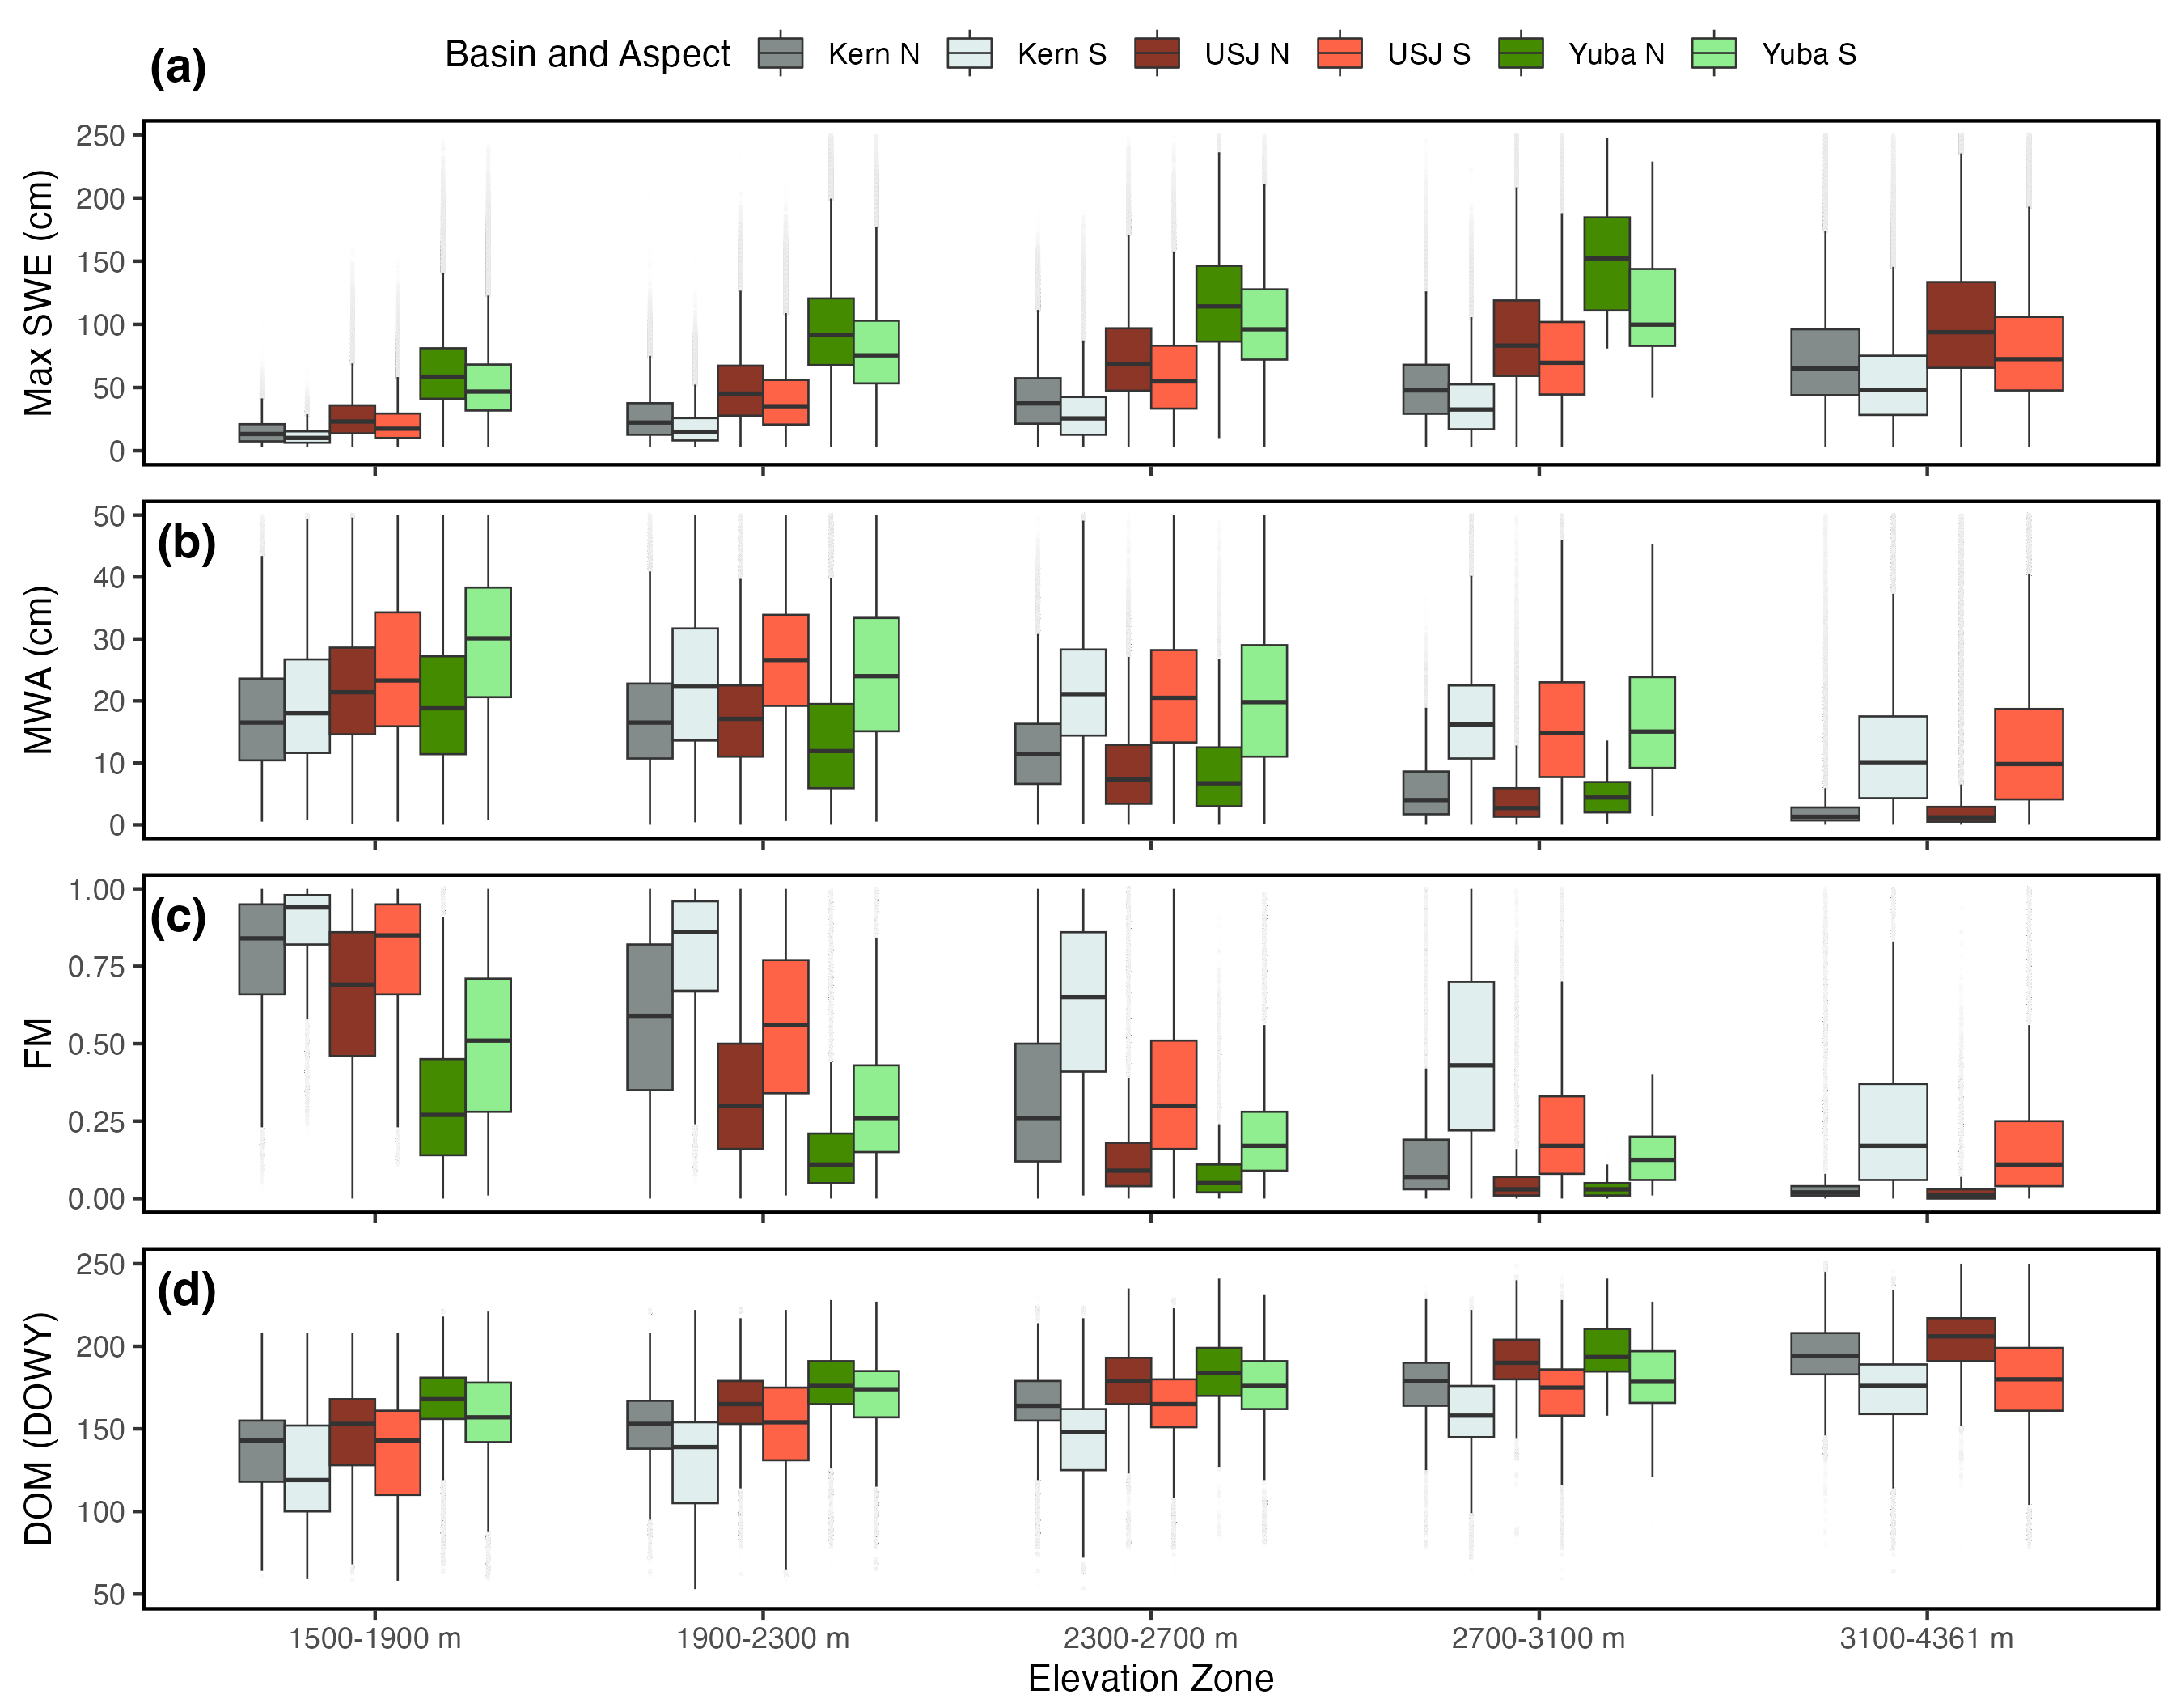
\includegraphics[width=\textwidth]{figures/ch2_figs/snow4_boxplot_v5.png}
\caption{Boxplots for \textbf{(a)} MSWE, \textbf{(b)} MWA, \textbf{(c)} FM, \textbf{(d)} DOM, for the 32-year study period. The data are grouped by the five EZs and colored the three basins: Kern (gray), USJ (orange), Yuba (green). The colors shading represents north-facing (darker) and south-facing (lighter) slopes for the respective basin.}
\label{fig:snow_boxplots}
\end{figure*}


For all of the snow metrics in all three basins, there are marked differences between the north and south-facing slopes (Fig.~\ref{fig:snow_boxplots}). Overall the Kern, which is the southern most basin, has the greatest mean FM values (Fig.~\ref{fig:snow_boxplots}a) for all elevation bands when compared to the Yuba and the USJ. Additionally, it had the highest mean FM percent difference between south and north-facing slopes of 69.6~\%. Yet, shown in Fig. \ref{fig:met_boxplots} and Table \ref{tab:met_metric_table}, the Kern has either similar or colder T\textsubscript{mean} values (Fig. \ref{fig:met_boxplots}a) than the Yuba and the USJ. These differences are possibly explained by the insolation values in the Kern (Fig. \ref{fig:snow_boxplots}c) being greater by $\sim$15--25 $\mathrm{W~m}^{-2}$ across all EZs. 

Elevation trends are consistently observed across all three basins for each of the four metrics, although the magnitude of the differences varies incongruently among the basins. As expected, MSWE and DOM increase with elevation, while FM and MWA broadly decrease. The two midwinter ablation metrics (FM and MWA) impact both MSWE and DOM for all basins and EZs. Across the three basins, south-facing slopes reach DOM on average 16.1~d earlier, with the greatest mean difference of 25 d occuring in the USJ between 3100--4361~m. MSWE on north-facing slopes is on average 154~mm greater across all basins and EZs. North vs. south-facing disparities are amplified by increasing elevation, with a maximum difference of 467~mm in EZ4 of the Yuba.

For EZ4 (2700--3100~m) and EZ5 (3100--4361~m), the USJ and Kern showed particularly stark differences in both midwinter ablation metrics with respect to aspect. The mean FM and MWA values for the two basins in these elevation zones on north-facing slopes were 0.07 and 39~mm, respectively. In contrast, south-facing slopes had markedly higher values, with mean FM and MWA values of 0.29 and 151~mm. This means there is approximately 4 times more FM and MWA on south-facing slopes at elevations above 3100~m. Furthermore, the T\textsubscript{mean} values are below 0$^{\circ}$ for these areas.

Fig.~\ref{fig:aspec_mwa_fm_bp} shows boxplots of T\textsubscript{mean} split into 0.5 C$^{\circ}$ bins plotted against FM (left) and MWA (right) for the three study basins. Across all basins and T\textsubscript{mean} values, south-facing slopes show greater FM and MWA values.  The Kern and USJ have higher elevations, and therefore large areas with cold season T\textsubscript{mean} values below 0~$^{\circ}$C, in the places with T\textsubscript{mean} at or below $-$2~$^{\circ}$C we so almost midwinter ablation. 

For the gridMET derived metrics (T\textsubscript{mean}, RH***, insolation) there are no significant difference between the north-facing and south-facing slopes (Figure \ref{fig:met_boxplots}.a--c). This makes sense considering gridMET's native 4~km spatial resolution, thus not capturing the topographic heterogeneity of the 90~m SNSR data. CS insolation shows vast differences in the amount insolation received by the two aspects. Across all basins and EZs, south-facing slopes have a mean daily value of 234 $\mathrm{W~m}^{-2}$, while north-facing's is 43 $\mathrm{W~m}^{-2}$. Since these are static clear sky estimates, the values say consistent across the three study basins and EZs.

\begin{table}[htbp]
\centering
\caption{The mean values of the MWSE, DOM, FM, and FM for the three study basins. Each basin is split into north-facing (NF) and south-facing (SF) with the difference between the two also shown.}
\label{tab:snow_metric_table}
\tiny % Reduce font size to \small
\begin{tabular}{llrrrrrrrrrrrr}
\toprule
& & \multicolumn{3}{c}{MSWE (mm)} & \multicolumn{3}{c}{DOM (DOWY)} & \multicolumn{3}{c}{FM} & \multicolumn{3}{c}{MWA (mm)} \\
\midrule
Basin & EZ & NF & SF & Diff & NF & SF & Diff & NF & SF & Diff & NF & SF & Diff \\
\midrule
Kern & 1500--1900 m & 151 & 116 & -35 & 138 & 127 & -11 & 0.78 & 0.87 & 0.09 & 178 & 201 & 23 \\
Kern & 1900--2300 m & 269 & 191 & -78 & 149 & 133 & -16 & 0.58 & 0.79 & 0.21 & 171 & 238 & 67 \\
Kern & 2300--2700 m & 414 & 301 & -113 & 164 & 143 & -21 & 0.34 & 0.62 & 0.28 & 119 & 222 & 103 \\
Kern & 2700--3100 m & 518 & 375 & -143 & 178 & 156 & -22 & 0.15 & 0.47 & 0.32 & 56 & 177 & 121 \\
Kern & 3100--4361 m & 744 & 555 & -189 & 195 & 173 & -22 & 0.04 & 0.25 & 0.21 & 25 & 123 & 98 \\
USJ & 1500--1900 m & 267 & 219 & -48 & 146 & 136 & -10 & 0.65 & 0.78 & 0.13 & 218 & 262 & 44 \\
USJ & 1900--2300 m & 505 & 411 & -94 & 163 & 149 & -14 & 0.35 & 0.56 & 0.21 & 172 & 282 & 110 \\
USJ & 2300--2700 m & 745 & 614 & -131 & 178 & 162 & -16 & 0.14 & 0.35 & 0.21 & 87 & 221 & 134 \\
USJ & 2700--3100 m & 927 & 771 & -156 & 191 & 172 & -19 & 0.06 & 0.24 & 0.18 & 43 & 170 & 127 \\
USJ & 3100--4361 m & 1068 & 808 & -260 & 204 & 179 & -25 & 0.03 & 0.18 & 0.15 & 31 & 133 & 102 \\
Yuba & 1500--1900 m & 637 & 531 & -106 & 166 & 153 & -13 & 0.31 & 0.5 & 0.19 & 203 & 335 & 132 \\
Yuba & 1900--2300 m & 960 & 809 & -151 & 176 & 168 & -8 & 0.15 & 0.31 & 0.16 & 136 & 272 & 136 \\
Yuba & 2300--2700 m & 1210 & 1020 & -190 & 184 & 174 & -10 & 0.08 & 0.21 & 0.13 & 85 & 221 & 136 \\
Yuba & 2700--3100 m & 1660 & 1193 & -467 & 196 & 178 & -18 & 0.04 & 0.15 & 0.11 & 61 & 178 & 117 \\
\bottomrule
\end{tabular}
\end{table}


\begin{figure*}[t]
\centering
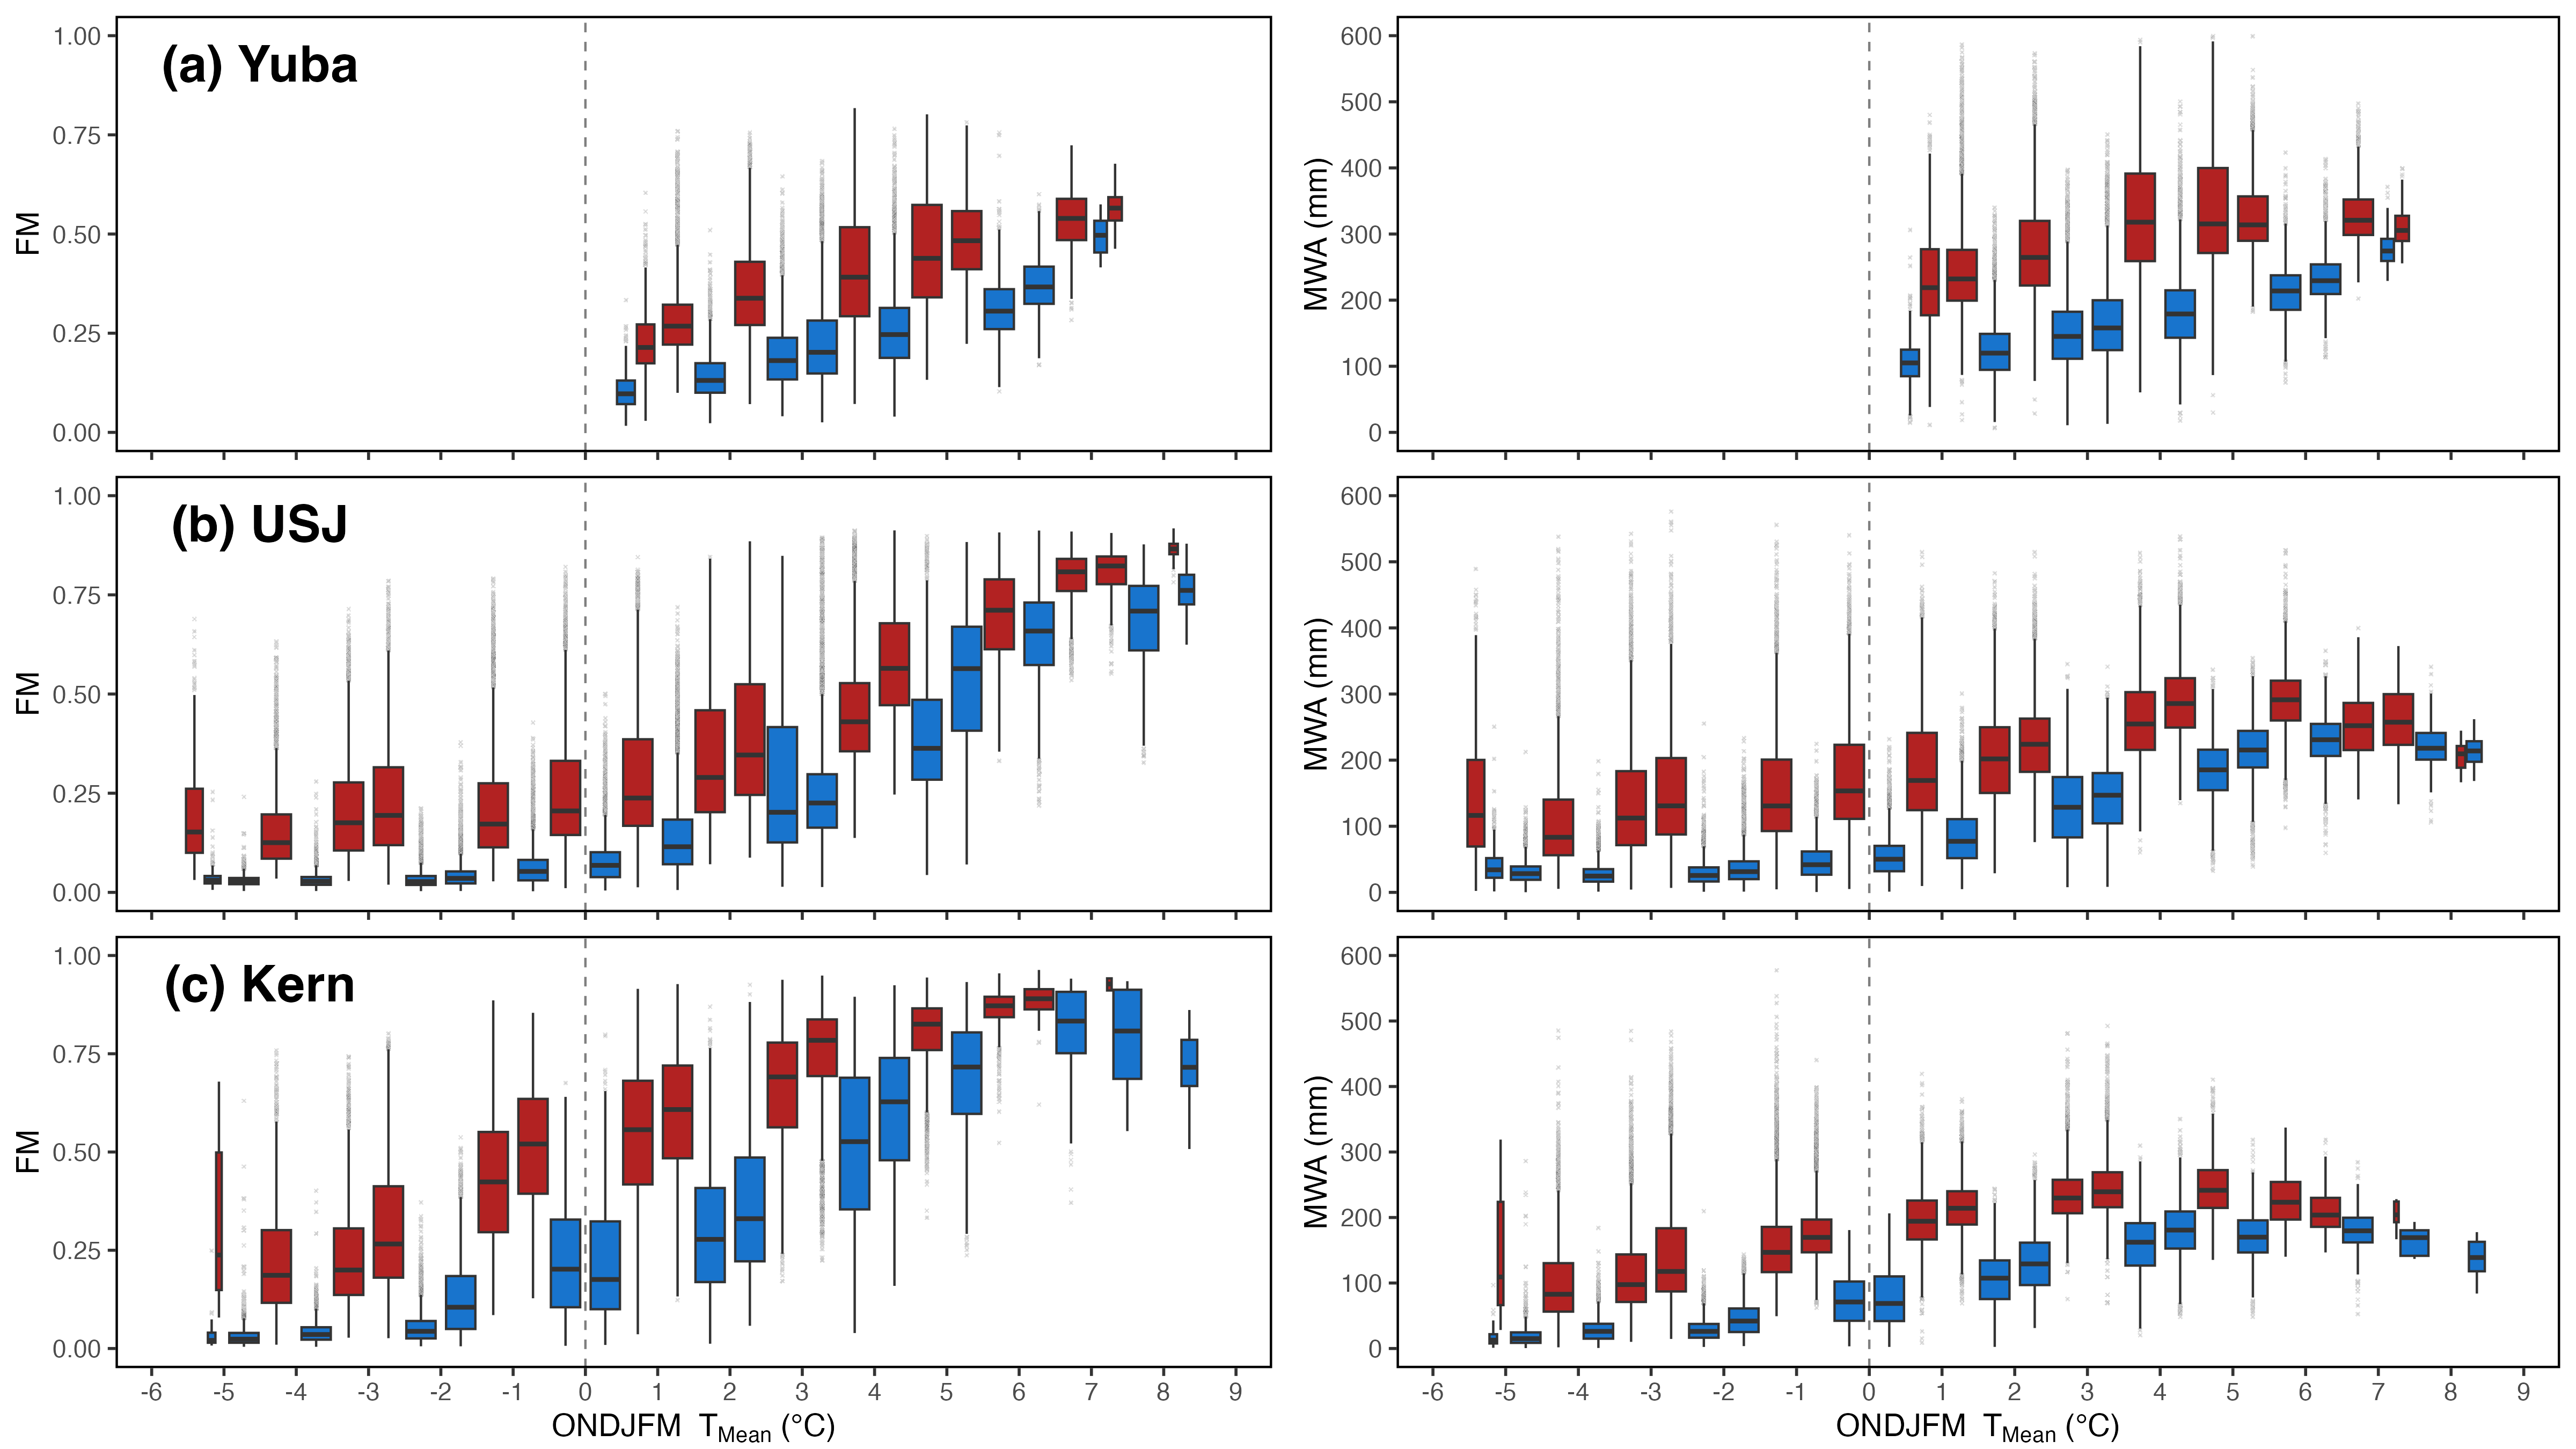
\includegraphics[width=\textwidth]{figures/ch2_figs/aspect_temp_mwa_fum_full_boxplots_v2.png}
\caption{Boxplots comparing FM (left) and MWA (right) on north-facing (blue) and south-facing (red) slopes for the \textbf{(a)} Yuba, \textbf{(b)} USJ, \textbf{(c)} Kern.}
\label{fig:aspec_mwa_fm_bp}
\end{figure*}

\begin{figure*}[h]
\centering
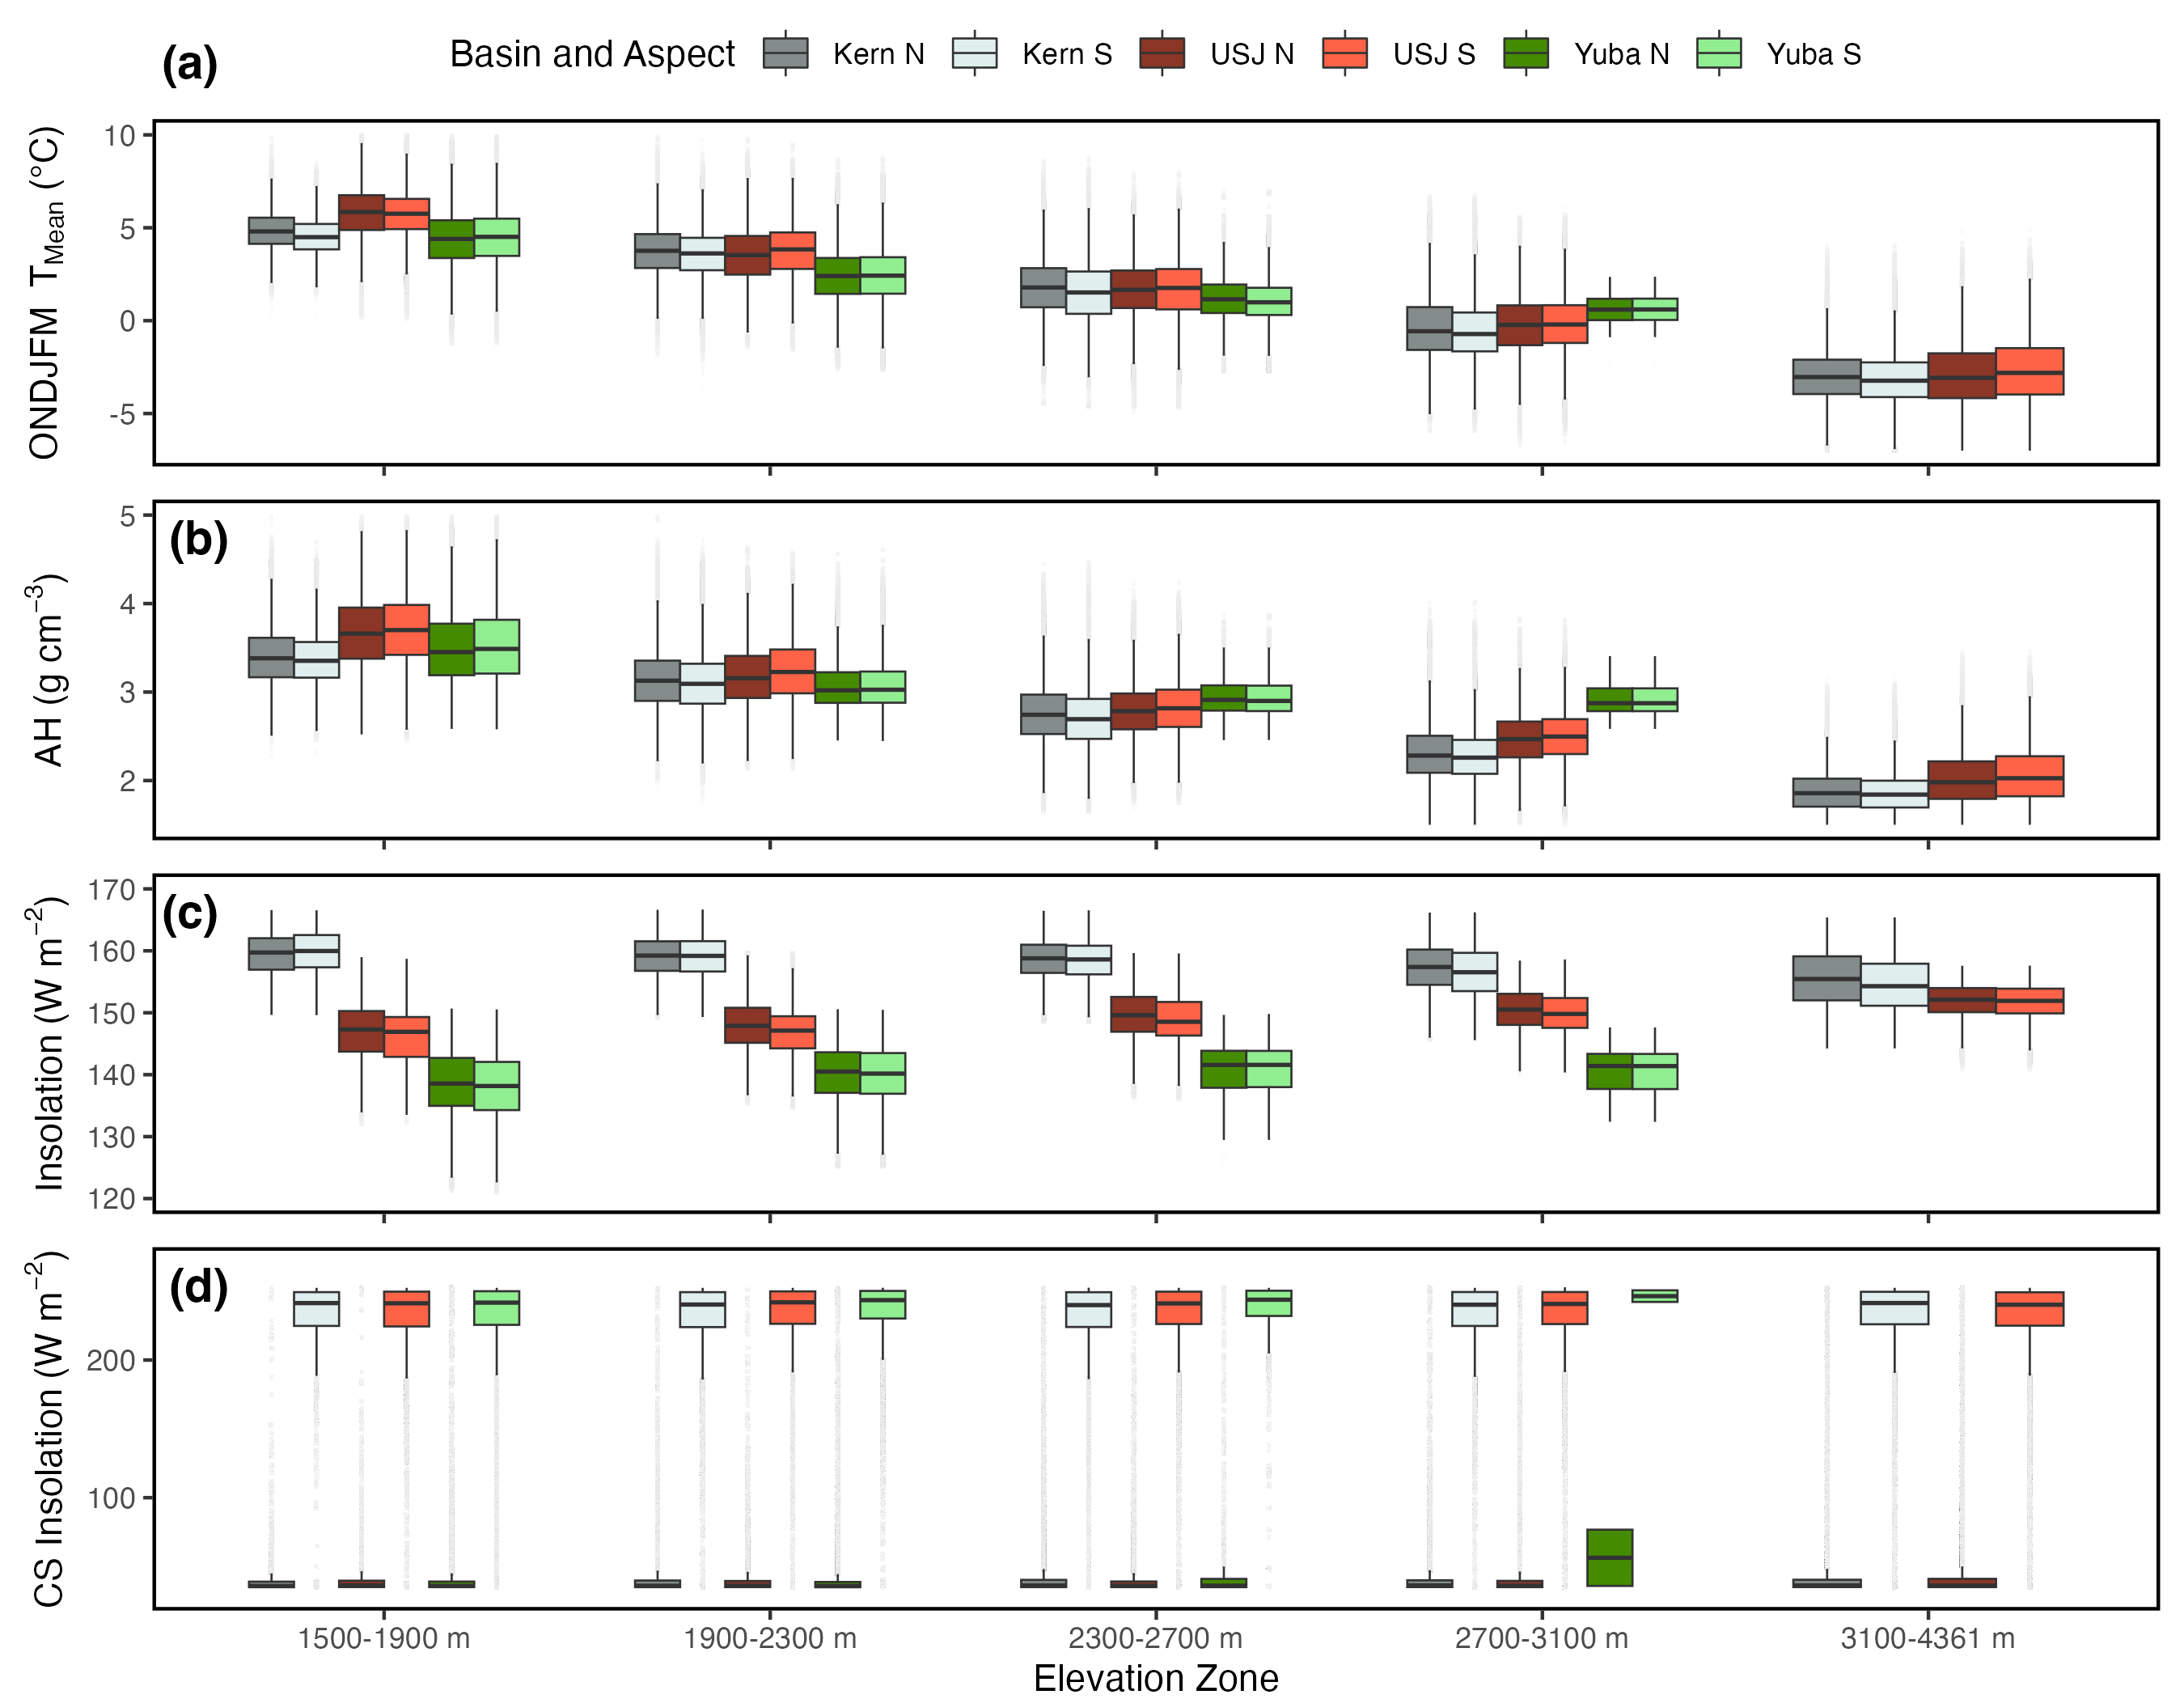
\includegraphics[width=\textwidth]{figures/ch2_figs/met4_boxplot_v4.png}
\caption{ Boxplots for \textbf{(a)} T\textsubscript{mean}, \textbf{(b)} AH, \textbf{(c)} insolation, and \textbf{(d)} CS insolation for the 32-year study period. The data are grouped by the five EZs and colored the three basins: Kern (gray), USJ (orange), Yuba (green). The colors shading represents north-facing (darker) and south-facing (lighter) slopes for the respective basin.}
\label{fig:met_boxplots}
\end{figure*}

\begin{table}[htbp]
\centering
\caption{******UPDATE:REMOVE AH****** The mean values of the T\textsubscript{mean}, AH, insolation, and CS insolation for the three study basins. Each basin is split into north-facing (NF) and south-facing (SF) with the difference between the two also shown.}
\label{tab:met_metric_table}
\tiny 
\begin{tabular}{llrrrrrrrrrrrr}
\toprule
& & \multicolumn{3}{c}{T\textsubscript{mean}} & \multicolumn{3}{c}{AH} & \multicolumn{3}{c}{Insolation} & \multicolumn{3}{c}{CS Insolation} \\
\midrule
Basin & EZ & NF & SF & Diff & NF & SF & Diff & NF & SF & Diff & NF & SF & Diff \\
\midrule
Kern & 1500-1900 m & 4.98 & 4.68 & -0.3 & 3.4 & 3.37 & -0.03 & 159 & 159 & 0 & 41 & 231 & 190 \\
Kern & 1900-2300 m & 3.86 & 3.68 & -0.18 & 3.14 & 3.1 & -0.04 & 159 & 158 & -1 & 41 & 232 & 191 \\
Kern & 2300-2700 m & 1.83 & 1.56 & -0.27 & 2.75 & 2.7 & -0.05 & 158 & 158 & 0 & 41 & 232 & 191 \\
Kern & 2700-3100 m & -0.39 & -0.55 & -0.16 & 2.31 & 2.28 & -0.03 & 157 & 156 & -1 & 41 & 233 & 192 \\
Kern & 3100-4361 m & -2.98 & -3.13 & -0.15 & 1.85 & 1.83 & -0.02 & 155 & 154 & -1 & 46 & 233 & 187 \\
USJ & 1500-1900 m & 5.83 & 5.78 & -0.05 & 3.67 & 3.7 & 0.03 & 147 & 146 & -1 & 40 & 232 & 192 \\
USJ & 1900-2300 m & 3.56 & 3.78 & 0.22 & 3.18 & 3.24 & 0.06 & 147 & 147 & 0 & 39 & 233 & 194 \\
USJ & 2300-2700 m & 1.64 & 1.68 & 0.04 & 2.79 & 2.82 & 0.03 & 149 & 148 & -1 & 40 & 234 & 194 \\
USJ & 2700-3100 m & -0.28 & -0.2 & 0.08 & 2.46 & 2.49 & 0.03 & 150 & 149 & -1 & 41 & 233 & 192 \\
USJ & 3100-4361 m & -2.92 & -2.7 & 0.22 & 2.01 & 2.05 & 0.04 & 151 & 151 & 0 & 46 & 232 & 186 \\
Yuba & 1500-1900 m & 4.42 & 4.52 & 0.1 & 3.5 & 3.53 & 0.03 & 138 & 137 & -1 & 41 & 231 & 190 \\
Yuba & 1900-2300 m & 2.45 & 2.47 & 0.02 & 3.07 & 3.07 & 0 & 140 & 140 & 0 & 41 & 236 & 195 \\
Yuba & 2300-2700 m & 1.22 & 1.09 & -0.13 & 2.94 & 2.93 & -0.01 & 140 & 140 & 0 & 47 & 236 & 189 \\
Yuba & 2700-3100 m & 0.69 & 0.7 & 0.01 & 2.91 & 2.91 & 0 & 140 & 140 & 0 & 56 & 246 & 190 \\
\bottomrule
\end{tabular}
\end{table}

\hypertarget{ch2-results-3}{\subsection{Snow metric climate sensitivity}\label{ch2-results-3}}

Fig.~\ref{fig:heat_map} displays the results of our Spearman correlations between FM on north and south-facing slopes and three meteorological variables: T\textsubscript{mean}, RH, and insolation. Overall, FM in the Yuba is highly sensitive to the three variables tested on both south-facing slopes in all EZs. For the three lowest EZs, spanning 1500--3100~m, a minimum of 90~\% of the land area shows significant relationships between FM and T\textsubscript{mean}. 

The Kern and the USJ display similar patterns for the various correlations; therefore, we group these basins together when reporting their results below. For the top two EZs (2700--4361~m) in the Kern and USJ, the T\textsubscript{mean} sensitivity on north and south-facing slopes diverges. Seen on the right side of Fig.~\ref{fig:heat_map}, the USJ and Kern have a mean of 14.5~\% of the area that is temperature sensitive, while south-facing slopes show a markedly greater mean value of 70~\%. In contrast, this relationship reverses for the EZ1 and EZ2, where north-facing slopes have a greater mean sensitive area (96~\%) while south-facings slopes shows much less significance (mean of 65 \%). We note that the low percentage areas of significant relationship in EZ1--2 does not mean low FM---these areas have the largest mean FM values of anywhere in the study---it just means the FM wasn't correlated to T\textsubscript{mean}.

-report results for RH and insolation


\begin{figure*}[h]
\centering
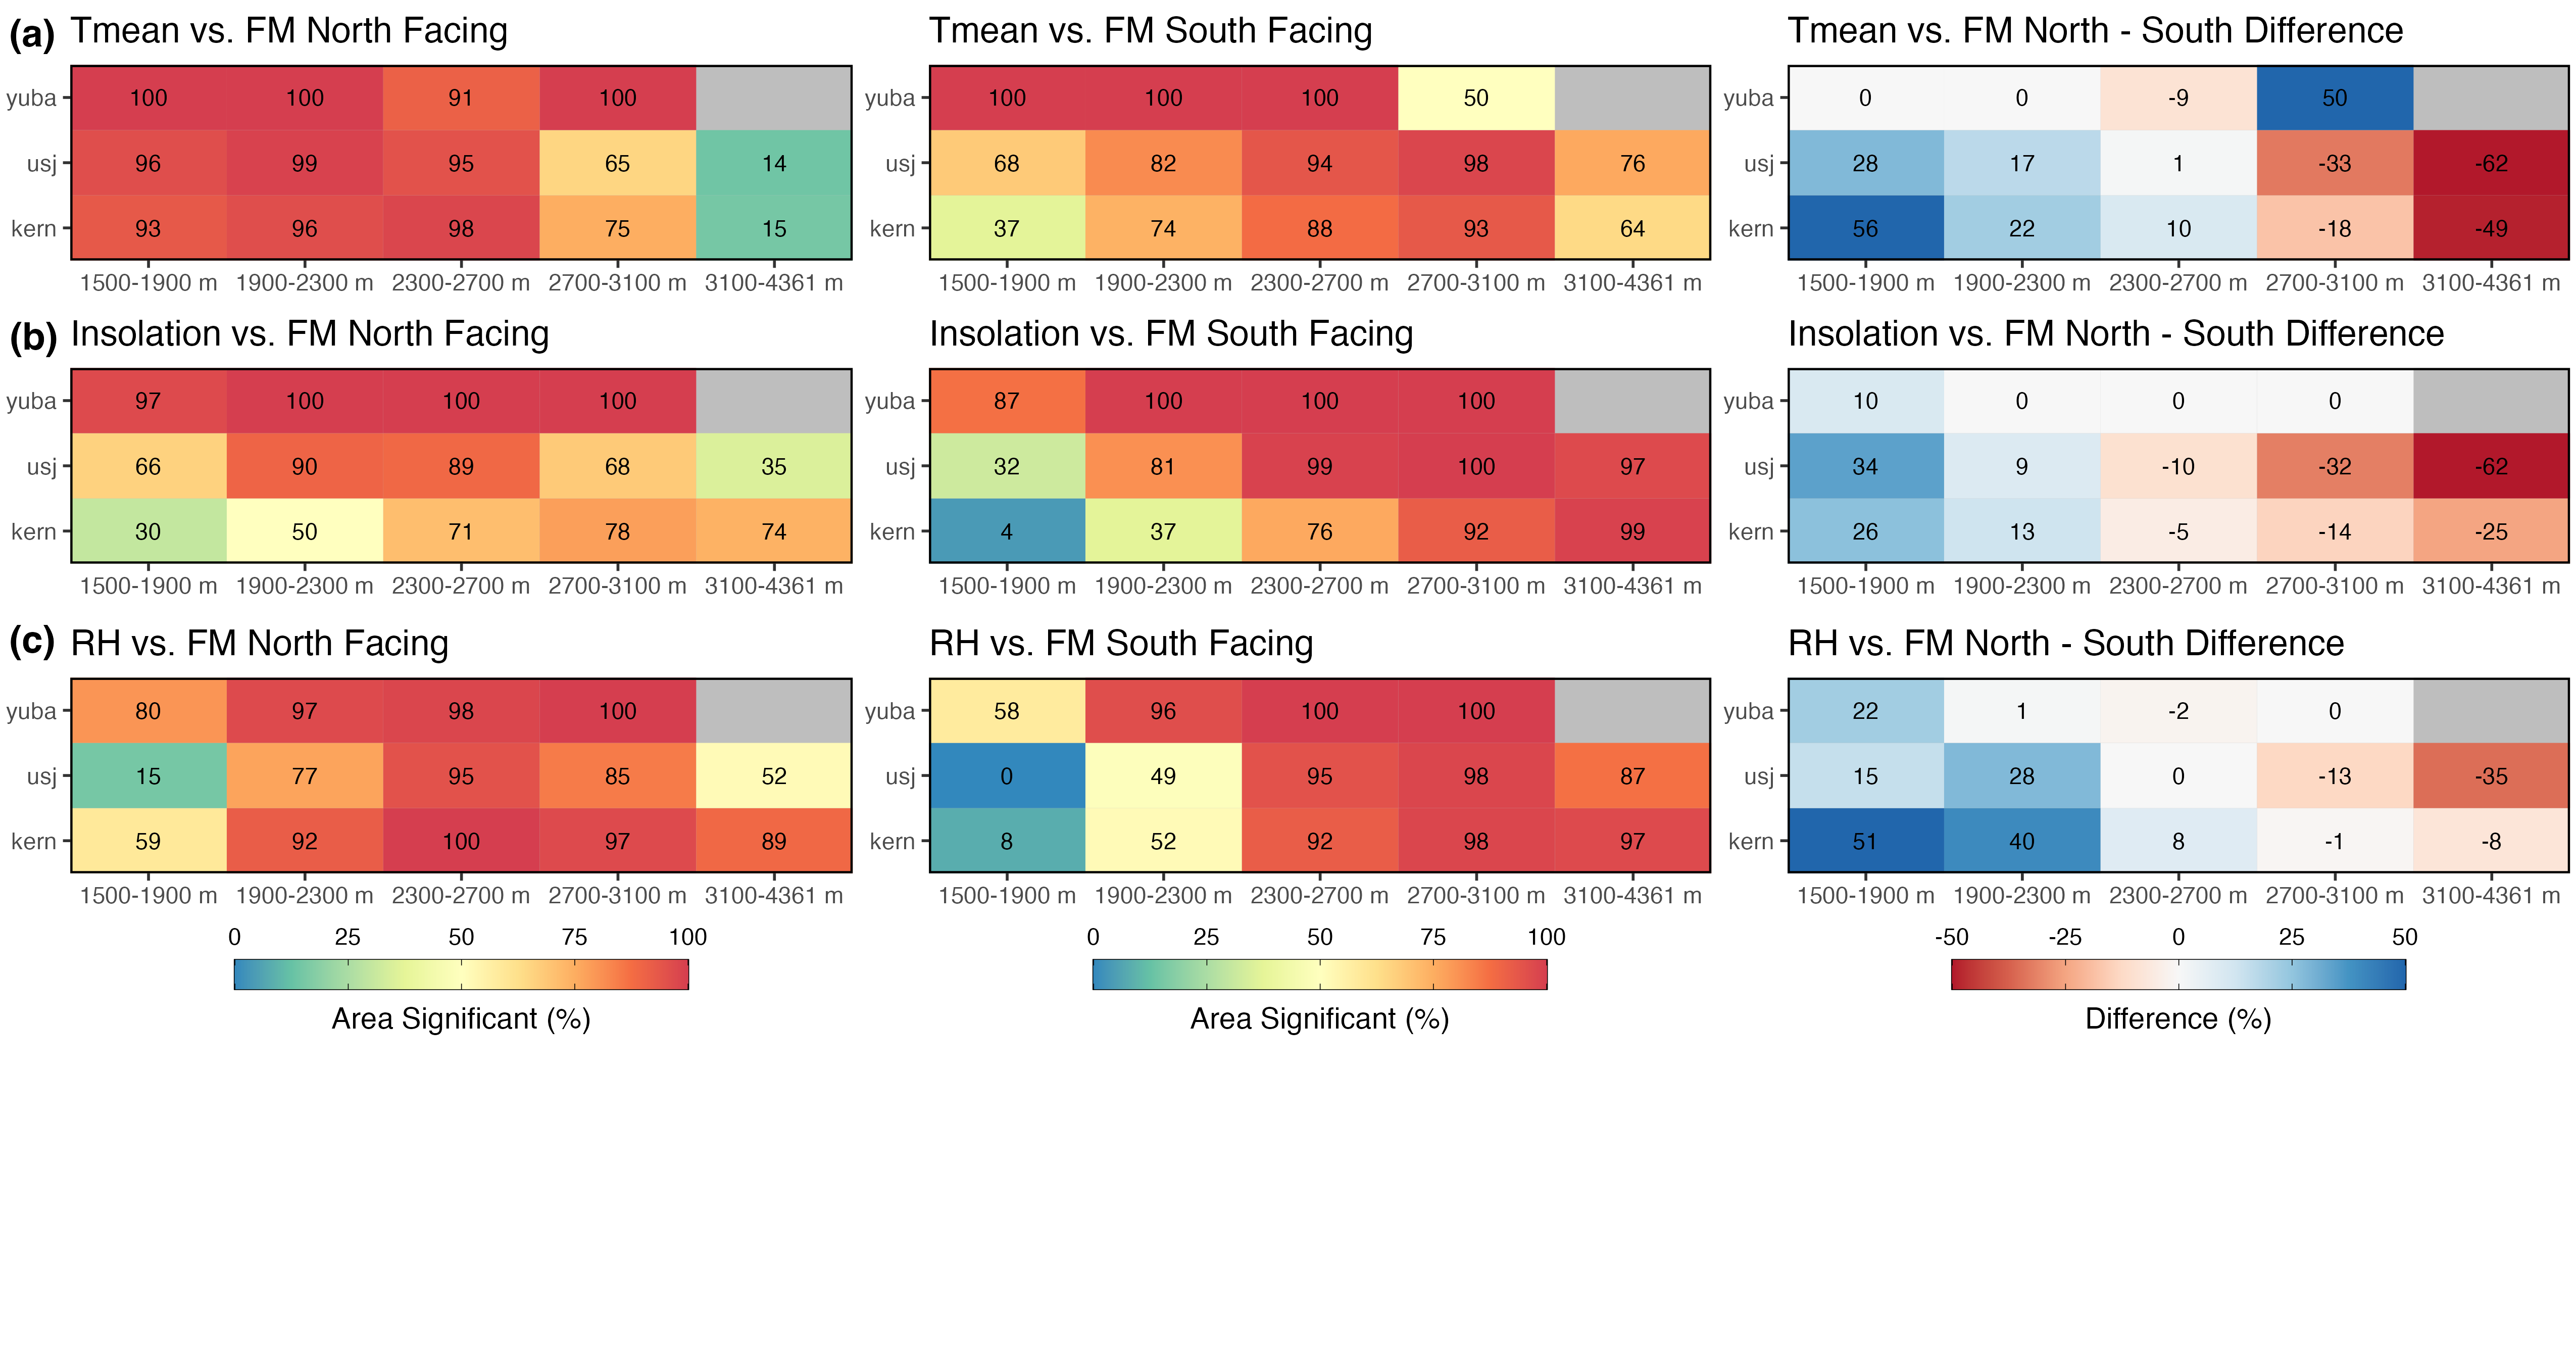
\includegraphics[width=\textwidth]{figures/ch2_figs/metvars_fm_heatmaps_v4.png}
\caption{Heat maps of the displaying percentage of area in each EZ with significant trends ($p < .05$) for \textbf{(a)} T\textsubscript{mean}, \textbf{(b)} RH, \textbf{(c)} insolation for the 32-year study period. The panels are split into north (left), south-facing (center) slopes, and the difference between the two (right). The color bars correspond to the values within a given panel. Elevation in the Yuba doesn't rise above 3100~m, shown by a gray value in the heatmap.}
\label{fig:heat_map}
\end{figure*}



%==============================================================================
%==============================================================================
%==============================================================================
\hypertarget{ch2-discussion}{\section{Discussion}\label{ch2-discussion}}


While south vs. north-facing slope patterns are well-established and visible throughout many mountain ranges across the globe, our study quantified these aspect-driven midwinter ablation variations with respect to T\textsubscript{mean} and elevation. As discussed when we compared midwinter ablation to elevation, the north vs. south-facing difference varies by basin and T\textsubscript{mean}. 

This makes them sensible heat-driven midwinter ablation for two reasons; T\textsubscript{mean} rises above 0~$^{\circ}$C less frequently, and when it does, the sensible heat flux goes to decreasing cold content and not ablating the snow.

Before we can have any melt, all cold content must be removed from the snowpack***. The primary control on snowpack cold content is the amount and temperature of snowfall (cite keith, 2018), with a negative energy balance being a secondary control. Additionally, degree-day models like SNOW17 use temperature as a proxy for the snowpack energy balance. The areas at high elevations (EZ4--5) have a greater amount of snowpack cold content as a result of greater total season snowfall and colder snowpacks. These two factors** make the high-elevation snowpack, especially north-facing slopes, less susceptible to melt. However, we showed that south-facing slopes at these higher elevations on average four times greater FM and MWA.  This suggests that insolation is a driving factor in high-elevation midwinter ablation. Conversely, the warmest T\textsubscript{mean} values have the most similar north and south-facing values. This suggests that at these warmer temperatures, which are lower elevation areas with shallower snowpacks, sensible heat flux is driving the melt and sublimation. 


%%%% 
-talk about hypsometry and the fact that much more area at low to mid elevations
-paragraph on temperature variation \citp{kapnickCausesRecentChanges2012}


At lower elevations, warmer snowpack temperatures lead to greater snow grain metamorphism and larger grain sizes (Colbeck refs). This leads to a secondary, amplifying effect: greater absorption of solar radiation in the near-infrared wavelengths by larger snow grains (wiscombe and warren, 1980, warren 1980). Moreover, midwinter ablation will increase the concentration of light absorbing impurities on the snowpack surface (hatchett, gleason, skiles/painter). In the Sierra Nevada, Hatchett et al. document the increase in frequency and length of mid winter dry spells and their interactions with post-fire black carbon on snowpacks in burned forests. 

%%% 
It's important to note the impacts of forest structure on snowpack energy balance and, therefore, snowpack evolution \citep{rothForestImpactsSnow2017}. Aspect is a key control on forest structure and composition \citep{pelletierWhichWayYou2018a}.  As shown by our CS insolation model, south-facing slopes receive $\sim$191 $\mathrm{W~m}^{-2}$ more direct solar radiation. Solar radiation is a primary driver for evaporation and sublimation at both the snow and soil surfaces (CITE), impacting plant available water, and therefore decreasing vegetation biomass on south-facing slopes \citep{zapata-riosInfluenceTerrainAspect2016}. Lower forest density allows more insolation to reach the snow surface. There are strong linkages and feedbacks among aspect, insolation, forest cover, and snow hydrology. However, when considering other energy balance components, forest-snow interactions are more complicated.  Both \citep{lundquistLowerForestDensity2013,rothForestImpactsSnow2017} showed that warmer, low-elevation forests can deplete snowcover whereas colder, higher elevation forests preserve snowpack. However, neither of those studies addressed the effects of aspect. A comprehensive evaluation of forest impacts on snow across north- and south-facing aspects is beyond the scope of this study.


north-facing slopes have denser vegetation, obstructing much of the insolation, therefore shielding. At the forest gap scale, these same north vs. south gap patterns are also seen (mussleman 2012, webb 2020). These driven forest patterns only 


\hypertarget{ch2-discussion-1}{\subsection{Limitations and future work}\label{ch2-discussion-1}}

% model validation 
Our study utilized 29 SNOTEL stations, primarily centered around Lake Tahoe, for the validation of the modeled snow metrics. We did not include the California Department of Water Resources (CADWR) snow pillows, as they have known data consistency issues. Future work should implement a quality-controlled version of these data into any model validation, as their geographic range representation of the entire Sierra. Additionally, as we've discussed in detail in this paper, in situ station-based measurements are photographically limited. However, they're the best available data source for large-scale model validation. Progressing in our understanding of snowpack will come from the synergistic use of in situ data, gridded snowpack energy balance models, and high-resolution satellite remote sensing of various snowpack properties (e.g., SWE, snow depth) \citep{flemingSNOTELSoilClimate2023}.

% temperature uncertainties
4~km gridMET data does not capture complex microclimates and aspect-driven variation in insolation or temperature. Previous work indicates that temperature patterns and lapse rates vary a small spatial scales in the Sierra \citep{lundquistSurfaceTemperaturePatterns2007}, with these variations not being accounted for in our analysis. Future work could implement the 800~m PRISM (Parameter-elevation Relationships on Independent Slopes Model) data \citep{dalyStatisticalTopographicModelMapping1994} for finer spatial resolutions. Yet, these data still are relatively coarse for mountain range applications. The gridMET insolation data shows both elevation and latitude-related trends. Our CS insolation model does not account for these variations.

%% wind and lopes
While not specifically parameterized in the SNSR, wind transport can substantially affect the distribution of snowpack \citep{winstralSpatialSnowModeling2002,marksSimulationTerrainForest2002}. Depending on the prevailing wind direction (westerly in the Sierra), lee-facing slopes tend to have deeper snowpack than scoured windward slopes. We were interested in investigating the relationships between radiation, temperature, and midwinter ablation, therefore omitted east and west-facing slopes from our analysis.

%% forest
The SNSR uses static land cover data from the National Land Cover Database (NLDC) \citep{homerConterminousUnitedStates2020}. This does not account for large-scale forest disturbances, mainly forest fires in the Sierra, which are increasing in both area and intensity in the seasonal snow zone \cite{koshkinWildfireImpactsWestern2022}. Future large-scale snow modeling work should look to implement temporally variable land cover characteristics, as forest fires have a significant impact on snow albedo \cite{gleasonCharredForestsIncrease2013} and the timing and magnitude of water resources \citep{williamsGrowingImpactWildfire2022}.

%% geogrpahy
We analyzed two west-facing basins (Yuba and USJ) and one south-facing basin in the Sierra. They do not encapsulate the full geographic and physiographic diversity of the range, therefore not capturing the full range of snow metric and meteorological values. We used subjective cut-offs for north-facing (315--45$^{\circ}$) vs. south-facing (135--215$^{\circ}$) aspects and for what is considered a slope (> 4$^{\circ}$).
% 
-paragraph on longwave and shortwave variation in a warming climate, ***there has been work that suggest SW may derecases as cloudover inceases***

-pomeroy (2009) long wave effects on cannopy

%==============================================================================
%==============================================================================
%==============================================================================
\hypertarget{ch2-conclusions}{\section{Conclusions}\label{ch2-conclusions}}

Our results show substantial differences between the four snow metrics for north and south-facing slopes, with patterns emerging with respect to EZ and basin. These findings further display the complexity and variability of mountain snowpacks even within the same basin and EZ. This suggests that physiographic relationships play an important role in the physical mechanisms governing snow ablation and accumulation. However, these factors are both spatial and temporally variable. 

\clearpage
\bibliographystyle{apalike}
\setstretch{1}
\bibliography{ch2.bib}
\setstretch{1.5}